\chapter{Caratteristiche pluviometriche dell’area di studio}\label{cap:pluviometriche}
\section{Curve di possibilità pluviometrica}
Dopo che si è eseguito un primo inquadramento della zona si procede con le elaborazioni dei dati dei massimi annuali degli scrosci e delle precipitazioni orarie ricavate dalla stazione pluviometrica di Laste a Trento.
Attraverso queste elaborazioni si pone l'obiettivo di determinare le curve di possibilità pluviometrica (CPP) a diversi tempi di ritorno $T_r$.
%(Tab.1 (a[mm/h alla n];n)).... svolte con il metodo di Gumbel momenti o minimi quadrati o massima verosimiglianza
Per la progettazione successiva si è scelto un tempo di ritorno pari a \SI{25}{anni}. 

Per graficare le CPP a tempo di ritorno assegnato occorre conoscere i parametri $a$ ed $n$ della loro equazione
\begin{equation}
    \label{eq:CPP}
    h = a\,(T_r) \, t_p ^{n}
\end{equation}

Tali parametri sono ottenuti attraverso una regressione lineare tra le altezze di pioggia $h_c (T_r)$ e le durate di intensità di pioggia $t_p$. 
I parametri $a$ ed $n$ sono rispettivamente il coefficiente angolare e l'intercetta di tale regressione, visualizzata in scala logaritmica a base 10. 

Per calcolare le altezze di pioggia $h_c (T_r)$ si è fatto uso di tre metodi diversi all'interno della distribuzione di Gumbel, ovvero la probabilità di non superamento 
\begin{equation}
  P(X\leq x) = \exp{\left[-\exp{\left[-x \right]} \right]}
\end{equation}
 dove $x = \alpha ( y - u)$ mentre $y$ è il vettore con i massimi annuali relativi ad una specifica durata di precipitazione, ottenuti dalla stazione pluviometrica.

I tre diversi metodi sono:
\begin{itemize}
\item dei momenti;
\item dei minimi quadrati;
\item della massima verosimiglianza.
\end{itemize}
Avendo quindi tre diversi parametri $\alpha$ ed $u$ (avendo usato tutti e tre i metodi), per scegliere la coppia di parametri migliore si è usato il test di Pearson o del $\chi ^2$.

%si può verificare la validità delle distribuzioni ottenute tramite il test di Pearson che consiste in un test di significatività statistica.
Fatto ciò si hanno i valori dell'altezza di precipitazione per ogni tempo di ritorno per una durata fissata. 
Eseguendo il calcolo per ogni durata ed elaborando la regressione lineare, si ottiene infine $a$ ed $n$ per poter graficare la CPP.

Nelle figure \ref{fig:ConfrontoMetodi} e \ref{fig:Pearson} viene mostrato la distribuzione di Gumbel e il relativo test di Pearson per una durata $t_p$ fissata di un'ora.
In figura \ref{fig:Regressione} è rappresentata la regressione lineare relativa ai due macro insiemi di durata (scrosci e orarie), ottenuta avendo fissato un tempo di ritorno di 25 anni. Da questo sono ottenuti i parametri $a$ ed $n$ riportati in tabella \ref{tab:parametriCPP} e da cui è stato rapresentato l'andamento delle due curve in figura \ref{fig:CPPFinale}.
\begin{table}[htbp]
    \centering
    \caption{Parametri $a$ ed $n$ per la costruzione della CPP}
    \label{tab:parametriCPP}
    \begin{tabular}{cS[table-format=2.12]S[table-format=1.12]}
            \toprule
            & $a$ & $n$ \\
            \midrule
            Scrosci & 34.890380507987 & 0.380264379496 \\
            Orarie & 32.123336325361 & 0.447173501027 \\ 
            \bottomrule
\end{tabular}
\end{table}

Da tale grafico si evince come si ottenga una maggiore altezza di precipitazione, dovuta agli scrosci, per le prime tre ore e mezza ($\hat{t}_p$) e poi le precipitazioni orarie superano gli scrosci. 
Per il seguente progetto, che riguarda un breve lasso di tempo, si prenderanno in considerazione soltanto gli scrosci. 

\begin{figure}[htbp]
    \centering
    \begin{tikzpicture}
        \begin{axis}[
            height=10cm,
            width=\textwidth,
            grid=major,
            legend pos={south east},
            xlabel=$h \, \si{[\milli\metre]}$,
            ylabel={$F, P(X\leq x)$},
            ytick = {0,0.2,0.4,0.6,0.8,1},
            %title= \emph{Vasca 2 posta a monte della condotta C21},
            /pgf/number format/.cd,
            use comma,
            1000 sep={\,}
        ]
        \addplot +[mark=*,only marks,color=green!60!black,mark options = {solid, fill=green!60!black}] table[x index=0,y index=1,header=false] {IMG/DaPython/curve__orario_1hfrequenza.txt};
        \addplot +[mark=none,style=solid,color=orange] table[x index=0,y index=1,header=false] {IMG/DaPython/curve__orario_1hmetodi.txt};
        \addplot +[mark=none,style=solid,color=magenta] table[x index=0,y index=2,header=false] {IMG/DaPython/curve__orario_1hmetodi.txt};
        \addplot +[mark=none,style=solid,color=cyan] table[x index=0,y index=3,header=false] {IMG/DaPython/curve__orario_1hmetodi.txt};
        \legend{Frequenza campionaria, Gumbel (Momenti), Gumbel (Minimi Quadrati), Gumbel (Massima Verosimiglianza)} 
        \node at (axis cs:9.7,0.9) [anchor=south west] {Durata \SI{1}{\hour}};   

        \end{axis}
    \end{tikzpicture}
    \caption{Confronto (a durata fissata) tra la frequenza campionaria e la probabilità di non superamento con i tre metodi della distribuzione di Gumbel}
    \label{fig:ConfrontoMetodi}
\end{figure}

\begin{figure}[htbp]
    \centering
    \begin{tikzpicture}
        \begin{axis}[
            height=10cm,
            width=\textwidth,
            grid=major,
            legend pos={south east},
            xlabel=$T_r \, \si{[anni]}$,
            ylabel=$h \, \si{[\milli\metre]}$,
            %ytick = {0,0.1,0.2,0.3,0.4,0.5,0.6,0.7,0.8,0.9,1},
            %title= \emph{Vasca 2 posta a monte della condotta C21},
            /pgf/number format/.cd,
            use comma,
            1000 sep={\,}
        ]
        \addplot +[mark=*,only marks,color=pantone186,mark options = {solid, fill=pantone186}] table[x index=0,y index=1,header=false] {IMG/DaPython/person__orario_1h.txt};
        \legend{{$t_p = \SI{1}{\hour}$}}    
        \end{axis}
    \end{tikzpicture}
    \caption{Andamento dell'altezza di precipitazione $h$ in funzione dei tempi di ritorno $T_r$ ottenuta dal test di Paerson per una durata $t_p$ fissata}
    \label{fig:Pearson}
\end{figure}

\begin{figure}[htbp]
    \centering
    \begin{tikzpicture}
    \begin{groupplot}[
            group style={
            %group name=my plots,
            group size=2 by 1
            %ylabels at=edge left
            },
            %restrict x to domain=-0:1.5,
            height=6cm,
            width=0.5\textwidth,
            xlabel=$t_p$ \si{[\hour]},
            ylabel=$h$  \si{[\milli\metre]},
            grid=major,
            xmode=log,
            ymode=log,
            %log ticks with fixed point,
            tick label style={
                /pgf/number format/.cd,
                use comma,
                1000 sep={\,}},
            ]
        \nextgroupplot[
            title=Scrosci]
        \addplot +[mark=none,style=solid,color=blue] table[x index=0,y index=1,header=false] {IMG/DaPython/RegressioneScrosci.txt};
        \nextgroupplot[
            title=Orarie,
            ylabel=\empty]
        \addplot +[mark=none,style=solid,color=red] table[x index=0,y index=1,header=false] {IMG/DaPython/RegressioneOrarie.txt};
    \end{groupplot}
    \end{tikzpicture}
    \caption{Regressione lineare delle altezze di pioggia con un $T_r =$ 25 anni in scala logaritmica}
    \label{fig:Regressione}
\end{figure}

\begin{figure}[htbp]
    \centering
    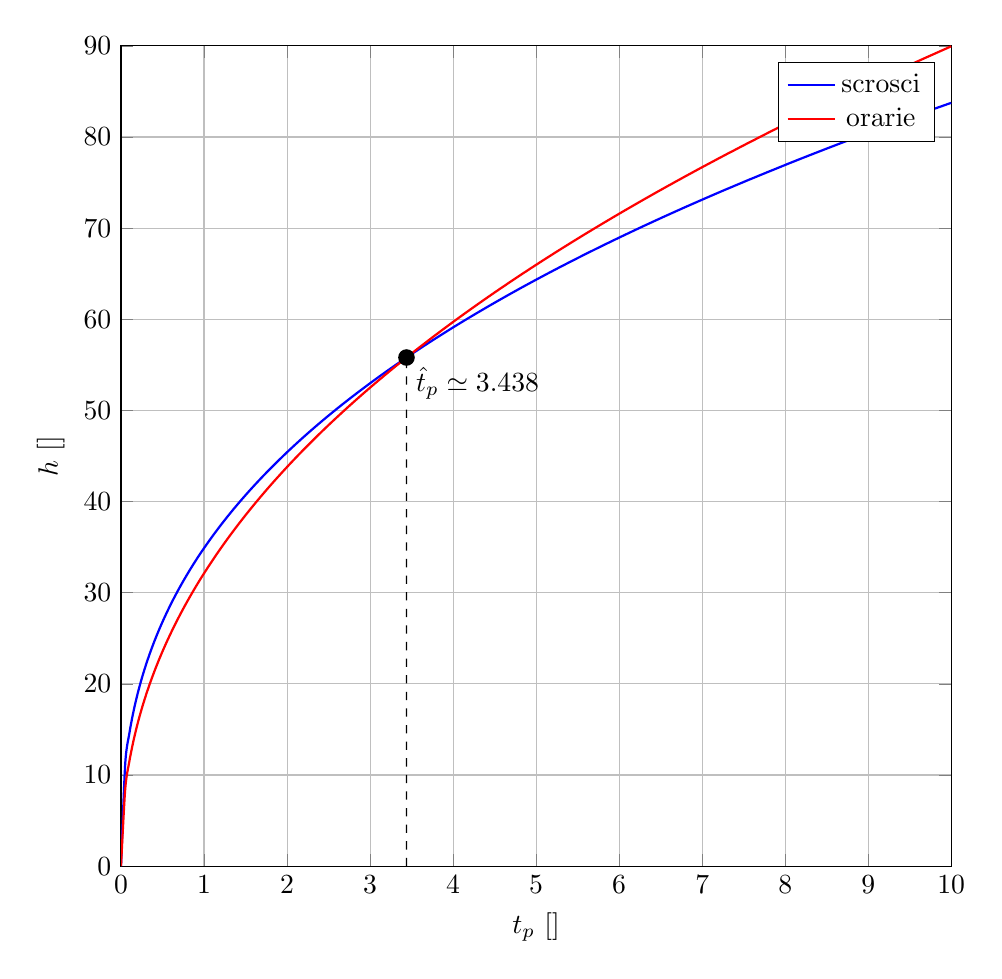
\begin{tikzpicture}
        \begin{axis}[
            xmin = 0, xmax = 10,
            ymin = 0, ymax = 90,
            xtick distance = 1,
            ytick distance = 10,
            height=12cm,
            width=\textwidth,
            grid=major,
            xlabel=$t_p$ \si{[\hour]},
            ylabel=$h$  \si{[\milli\metre]},
            %xtick = {0,0.5,1,1.5,2,2.5,3,3.5,4},
            %title= ,
            /pgf/number format/.cd,
            use comma,
            1000 sep={\,}
        ]
        \addplot [
            domain = 0:10,
            samples = 200,
            smooth,
            thick,
            blue,
        ]{34.890380507986976*x^0.38026437949595393};
        \addplot [
            domain = 0:10,
            samples = 200,
            smooth,
            thick,
            red,
        ]{32.123336325360924*x^0.4471735010272544};
        \legend{scrosci, orarie};
        
        \draw[black,dashed] (3.438155,0) -- (3.4381,55.80218)
        node[anchor=north west] {$\hat{t}_p \simeq \SI{3.438}{\hour}$};
        \fill[] (3.4381,55.80218) circle (3pt);
        \end{axis}
    \end{tikzpicture}
    \caption{Curve di possibilità pluviometrica con i parametri $a$ ed $n$ ricavati dalla regressione logaritmica e sostituiti nell'equazione \ref{eq:CPP} con $T_r$ di 25 anni}
    \label{fig:CPPFinale}
\end{figure}